% Generated 2020-07-27 15:21:27 +0530
\subsection{Sensor} \label{sec:Sensor}

{term:Sensor} is a unique type of a piece of equipment.  A {term:Sensor} is typically comprised of two major components: a {term:sensor unit} that provides signal processing, conversion, and communications and the {term:sensing elements} that provides a signal or measured value.

The {term:sensor unit} is modeled as a {term:Lower Level} {block:Component} called {block:Sensor}.  The {term:sensing element} may be modeled as a {block:Composition} element of a {block:Sensor} element and the measured value would be modeled as a {block:DataItem} (See {ref:Listing of Data Items} for more information on {block:DataItem} elements).  Each {term:sensor unit} may have multiple {term:sensing elements}; each representing the data for a variety of measured values.

Example:  A pressure transducer could be modeled as a {block:Sensor} ({block:Component}) with a {property:name} = {cite:Pressure Transducer B} and its measured value could be modeled as a {block:PRESSURE} type {block:DataItem}.

While a {term:Sensor} may be modeled in the {term:normalfont XML} document in different ways, it will always be modeled to associate the information measured by each {term:sensor element} with the {term:Structural Element} to which the measured value is most closely associated.   

\subsubsection{Sensor Data}

The most basic implementation of a sensor occurs when the {term:sensing element} itself is not identified in the data model, but the data that is measured by the {term:sensing element} is provided as a data item associated with a {block:Component}.  An example would be the measured value of the temperature of a spindle motor.  This would be represented as a {block:DataItem} called {block:TEMPERATURE} that is associated with the {block:Rotary} type axis element called "C" as shown in {ref:example-of-sensing-element}:

\newpage 

\begin{lstlisting}[firstnumber=1,escapechar=|,%
    caption={Example of Sensing Element provided as data item associated with a Component}, label={lst:example-of-sensing-element}]
<Components>
    <Axes
        <Components>
            <Rotary id="c" name="C">
                <DataItems>
                    <DataItem type="TEMPERATURE" 
                        id="ctemp" category="SAMPLE" 
                        name="Stemp" units="DEGREE"/>
                </DataItems>
            </Rotary>
        </Components>
    </Axes>
</Components>
\end{lstlisting}

A sensor may measure values associated with any {block:Component} or {block:Device} element.   Some examples of how sensor data may be modeled are represented in {ref:sensor-data-associations}:

\begin{figure}[ht]
  \centering
  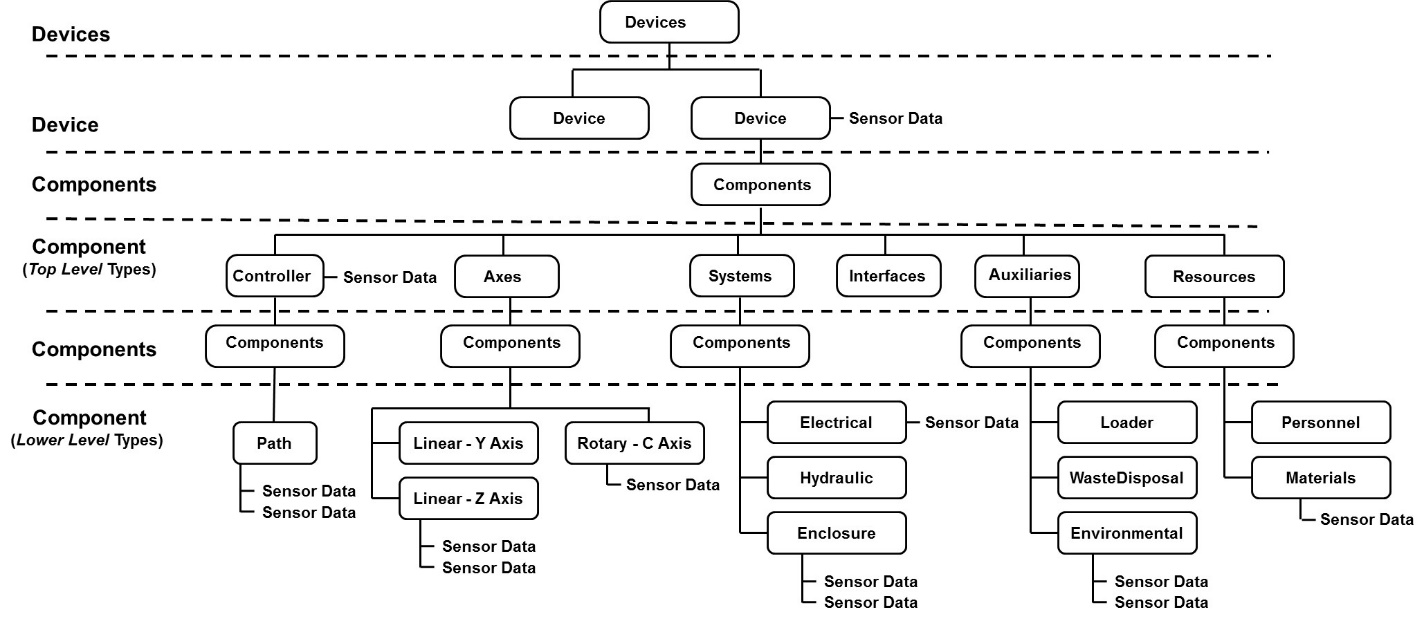
\includegraphics[width=.75\textwidth]{figures/sensor-data-associations.png}
  \caption{Sensor Data Associations}
  \label{fig:sensor-data-associations}
\end{figure}

\subsubsection{Sensor Unit}
\label{sec:Sensor Unit}

A {term:sensor unit} is an intelligent piece of equipment that manages the functions of one or more {term:sensing elements}.

Typical functions of the {term:sensor unit} include:

\begin{itemize}
\item convert low level signals from the {term:sensing elements} into data that can be used by other pieces of equipment.  (Example:  Convert a non-linear millivolt signal from a temperature sensor into a scaled temperature value that can be transmitted to another piece of equipment.)

\item process {term:sensing element} data into calculated values.  (Example:  temperature sensor data is converted into calculated values of average temperature, maximum temperature, minimum temperature, etc.)

\item provide calibration and configuration information associated with each {term:sensing element}

\item monitor the health and integrity of the {term:sensing elements} and the {term:sensor unit}.  (Example:  The {term:sensor unit} may provide diagnostics on each {term:sensing element} (e.g., open wire detection) and itself (e.g., measure internal temperature of the {term:sensor unit}).
\end{itemize}

Depending on how the {term:sensor unit} is used, it may be considered as either an independent piece of equipment and modeled in the {term:normalfont XML} document as a {block:Device}, or it may be modeled as a {term:Top Level} {block:Component} called {block:Sensor} if it is integral to a piece of equipment.

A {block:Sensor} **\may** have its own {block:uuid} so it can be tracked throughout its lifetime.

The following examples demonstrate how a {term:Sensor} may be modeled in the {term:normalfont XML} document differently based on how the {term:Sensor} functions within the overall piece of equipment

Example\#1:   If the {block:Sensor} provides vibration measurement data for the spindle on a piece of equipment, it could be modeled as a {block:Sensor} for rotary axis named C.

\begin{lstlisting}[firstnumber=1,escapechar=|,%
    caption={Example of Sensor for rotary axis}, label={lst:example-of-sensor}]
<Components>
  <Axes
    <Components>
      <Rotary id="c" name="C">
        <Components>
          <Sensor id="spdlm" name="Spindlemonitor">
            <DataItems>
              <DataItem type="DISPLACEMENT" id="cvib"
                category="SAMPLE" name="Svib" 
                units="MILLIMETER"/>
            </DataItems>
          </Sensor >
        <Components>
      </Rotary>
    </Components>
  </Axes>
</Components>
\end{lstlisting}

Example\#2:   If a {block:Sensor} provides measurement data for multiple {block:Component} elements within a piece of equipment and is not associated with any particular {block:Component} element, it **\may** be modeled in the {term:normalfont XML} document as an independent {term:Lower Level} {block:Component} and the data associated with measurements are associated with their associated {block:Component} elements.

This example represents a {term:sensor unit} with two {term:sensing elements}, one measures spindle vibration and the other measures the temperature for the X axis.   The {term:sensor unit} also has a {term:sensing element} measuring the internal temperature of the {term:sensor unit}.

\begin{lstlisting}[firstnumber=1,escapechar=|,%
    caption={Example of Sensor Unit with Sensing Element}, label={lst:example-of-sensor-with-sensing-elements}]
<Device id="d1" uuid="HM1" name="HMC_3Axis">
  <Description>3 Axis Mill</Description>
  <Components>
    <Axes
      <Components>
        <Sensor id="sens1" name="Sensorunit">
          <DataItems>
            <DataItem type="TEMPERATURE" id="sentemp"
              category="SAMPLE" name="Sensortemp" 
              units="DEGREE"/> 
          </DataItems>
        </Sensor >
        <Rotary id="c" name="C">
          <DataItems>
            <DataItem type="DISPLACEMENT" id="cvib"
              %category="SAMPLE" name="Svib" 
              units="MILLIMETER">
                <Source componentId="sens1"/>
            <DataItem/>
          </DataItems>
        </Rotary>
        <Linear id="x" name="X">
          <DataItems>
            <DataItem type="TEMPERATURE" id="xt" 
              category="SAMPLE" name="Xtemp" 
              units="DEGREE">
                <Source componentId="sens1"/>
            <DataItem/>
          </DataItems>
        </Linear>
      <Components>
    </Axes>
  </Components>
</Device>
\end{lstlisting}

When a {block:Sensor} unit is modeled in the {term:normalfont XML} document as a {block:Component} or as a separate piece of equipment, it may provide additional configuration information for the {term:sensor elements} and the {term:sensor unit} itself.  

{block:Configuration} data provides information required for maintenance and support of the sensor.

{block:Configuration} data is only available when the {block:Sensor} unit is modeled as a {block:Component} or a separate piece of equipment. For details on the modeling of configuration data in the {term:normalfont XML} document, see {ref:Configuration for Component}.

When {block:Sensor} represents the {term:sensor unit} for multiple {term:sensing element}(s), each sensing element is represented by a {block:Channel}.   The {term:sensor unit} itself and each {block:Channel} representing one {term:sensing element} **\may** have its own configuration data.

{block:SensorConfiguration} can contain any descriptive content for a {term:sensor unit}.  This element is defined to contain mixed content and additional {term:normalfont XML} elements (indicated by the {block:any} element in {ref:sensorconfiguration-schema-diagram}) **\may** be added to extend the schema for {block:SensorConfiguration}.



\subsubsection{Channel}
  \label{sec:Channel}


When {block:Sensor} represents multiple {term:sensing elements}, each {term:sensing element} is represented by a {block:Channel} for the {block:Sensor}. 


\paragraph{Attributes of Channel}\mbox{}
\label{sec:Attributes of Channel}

\tbl{attributes of Channel} lists the attributes of \texttt{Channel}.

\begin{table}[ht]
\centering 
  \caption{Attributes of Channel}
  \label{table:attributes of Channel}
\tabulinesep=3pt
\begin{tabu} to 6in {|l|l|l|} \everyrow{\hline}
\hline
\rowfont\bfseries {Attribute} & {Type} & {Multiplicity} \\
\tabucline[1.5pt]{}
\texttt{name} & \texttt{NMTOKEN} & 0..1 \\
\texttt{number} & \texttt{NMTOKEN} & 1 \\
\end{tabu}
\end{table}
\FloatBarrier


Descriptions for attributes of \texttt{Channel}:

\begin{itemize}
\item \texttt{name} : The name of an element or a piece of equipment.
\item \texttt{number} : A unique identifier that will only refer to a specific {term:sensing element}.
\end{itemize}

\paragraph{Elements of Channel}\mbox{}
\label{sec:Elements of Channel}

\tbl{elements of Channel} lists the elements of \texttt{Channel}.

\begin{table}[ht]
\centering 
  \caption{Elements of Channel}
  \label{table:elements of Channel}
\tabulinesep=3pt
\begin{tabu} to 6in {|l|l|l|} \everyrow{\hline}
\hline
\rowfont\bfseries {Association Name} & {Element} & {Multiplicity} \\
\tabucline[1.5pt]{}
\texttt{CalibrationDate} & \texttt{dateTime} & 0..1 \\
\texttt{CalibrationInitials} & \texttt{string} & 0..1 \\
\texttt{NextCalibrationDate} & \texttt{dateTime} & 0..1 \\
\texttt{Description} & \texttt{Description} & 0..1 \\
\texttt{Channels} & \texttt{SensorConfiguration} & 1 \\
\end{tabu}
\end{table}
\FloatBarrier


Descriptions for elements of \texttt{Channel}:

\begin{itemize}
\item \texttt{CalibrationDate} : Date upon which the {term:sensor unit} was last calibrated to the {term:sensor element}.
\item \texttt{CalibrationInitials} : The initials of the person verifying the validity of the calibration data.
\item \texttt{NextCalibrationDate} : Date upon which the {term:sensor element} is next scheduled to be calibrated with the {term:sensor unit}.

\item \texttt{Description} : An element that can contain any descriptive content.
\item \texttt{Channels} : {block:Channels} {term:organizes} {block:Channel} elements.

\end{itemize}
\FloatBarrier

\subsubsection{SensorConfiguration}
  \label{sec:SensorConfiguration}


{block:SensorConfiguration} contains configuration information about a {block:Sensor}.


\paragraph{Elements of SensorConfiguration}\mbox{}
\label{sec:Elements of SensorConfiguration}

\tbl{elements of SensorConfiguration} lists the elements of \texttt{SensorConfiguration}.

\begin{table}[ht]
\centering 
  \caption{Elements of SensorConfiguration}
  \label{table:elements of SensorConfiguration}
\tabulinesep=3pt
\begin{tabu} to 6in {|l|l|l|} \everyrow{\hline}
\hline
\rowfont\bfseries {Association Name} & {Element} & {Multiplicity} \\
\tabucline[1.5pt]{}
\texttt{CalibrationDate} & \texttt{dateTime} & 0..1 \\
\texttt{CalibrationInitials} & \texttt{string} & 0..1 \\
\texttt{FirmwareVersion} & \texttt{string} & 1 \\
\texttt{NextCalibrationDate} & \texttt{dateTime} & 0..1 \\
\texttt{Channels} & \texttt{Channel} & 0..* \\
\end{tabu}
\end{table}
\FloatBarrier


Descriptions for elements of \texttt{SensorConfiguration}:

\begin{itemize}
\item \texttt{CalibrationDate} : Date upon which the {term:sensor unit} was last calibrated.
\item \texttt{CalibrationInitials} : The initials of the person verifying the validity of the calibration data.
\item \texttt{FirmwareVersion} : Version number for the sensor unit as specified by the manufacturer.

\item \texttt{NextCalibrationDate} : Date upon which the {term:sensor unit} is next scheduled to be calibrated.
\item \texttt{Channels} : {block:Channels} {term:organizes} {block:Channel} elements.

\end{itemize}
\FloatBarrier
